\chapter{Implementation}

The following chapter details a range of different experiments carried out to investigate and compare the performance of the different inference methods described in the previous chapter. 


\section{Technical Details}

The implementation this project can be found at the GitHub repository...\question{GitHub link?} 
The inference inference methods are primarily implemented using the PyTorch deep learning framework. In addtion, the training framework PyTorch Lightning is used. This provides a bunch of features, such as handling of different computational devices such as GPU, handling the different train, validation and test data splits, an extensive callback API and more. 

In order to effectively compare different methods of inference across different models and data, the implementation is broken into separable components:

The model definitions are defined in the \texttt{src/models} directory. These are implemented as PyTorch modules with some additional methods that are used by the other components. 
At a high level, they define some amount of trainable parameters $\theta$, as well as a mapping from input $x$ to output $y=f_\theta(x)$. 
They also define an observation model through $p(y|x, \theta)$ using the distribution objects provided by PyTorch. 

Data, $(x_i, y_i)$ is represented by PyTorch datasets, each defining a way to extract indiviual observations. These are combined with the  

Finally, the different inference methods are implemented as LightningModules. There are three different inference methods defined. The 

The 


\todo[inline]{Implemeting a common interface is important to demonstrating potential of mcmc/vi as plugin replacements for standard inference method. Every experiment can be carried out using configurations of the same script.}

\section{Simulated Experiments}

In order to verify the implementation of the methods, some simulation experiment out. 
The first experiment is a recreation of an experiment also carried out in the SGHMC paper, where they sample from a bimodal distribution with $\log p(x) \propto 2 x^2 - x^ 4$ with different configurations. 
First, the distribution is sampled from as is, using regular HMC. Then the batched dynamics in \cref{eq:sghmc-model} are simulated by adding simulated noise $\epsilon \sim \mathcal{N}(0, 4)$ to the gradient during the sampling process. 
The distributional assumptions of SGHMC are thus fulfilled exactly, and we may also use the known noise scale as the noise estimate for SGHMC. 
With this introduced noise we also investigate the naive approach to using HMC, both with and without using an MH step. 
The resulting sampled distributions can be seen in \cref{fig:synthetic}
\begin{figure}[htbp]
    \centering
    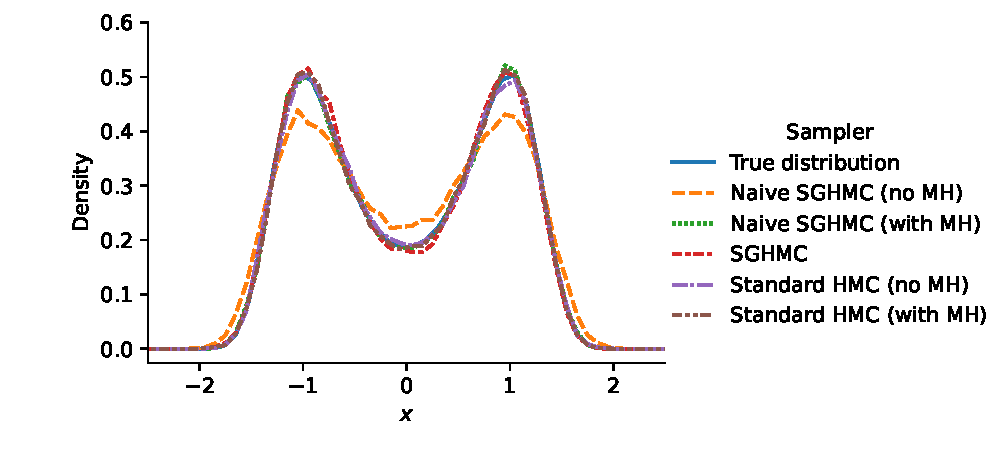
\includegraphics[width=0.9\textwidth]{Figures/synthetic.pdf}
    \caption{Samples from $\log p(x) \propto 2 x^2 - x^ 4$ for different sampling configurations}
    \label{fig:synthetic}
\end{figure}
These result seem to verify our that our implementation is correct. We also see that the sample distributions from both the standard HMC sampelr and the SGHMC sampler closely resembles the true distribution. 
The naive SGHMC sampler does seems to break down when no MH step is included, and since we also compare with regular HMC with no MH step, this demonstrates that it may not be purely down to omitting the MH step. 

If we include an MH step, the naive approach also seem to work, however we are not adding any noise to $E(\cdot)$ when performing the MH step, corresponding to calculating $E(\cdot)$ across the whole data set. 
This is impractical in the context of deep learning, but one could imagine an alternative naive HMC approach where an MH step based on each individual batch of data. 

This experiment also doesn't address whether noise the dynamics of \cref{eq:sghmc-model} are even reasonable as a model for the noise introduced through batching the gradient. 

In order to address these points, we perform an additional simulation experiment. 
This is also to demonstrate the relevance of the different methods in the context of MCMC inference.
We consider the polynomial model of $P(x) = -x + \frac{1}{2}x^2 + \frac{1}{3}x^3$, 
and with $\epsilon \sim \mathcal{N}(0, 1)$, 
consider a set learning points $y_i = P(x_i) + \epsilon$ for $i=1,\dots,15$, where $x_i$ are linearly spaced over the interval $[-3, 3)$ with a small amount of noise added. 
We then consider the problem of bayesian polynomial regression with known noise $\sigma=1$ and the regression model:
\begin{align*}
    P(x) = a_0 + a_1 x+a_2 x^2 + a_3 x^3
\end{align*}
where each parameter are given a $\mathcal{N}(0, 1)$ prior. The exact parameter posterior $p(a|x,y)$ for this regression problem is known, and can therefore be compared to the sampled distribution of the samplers. 
More specifically, three sampling strategies are considered, regular HMC conditioned on all data points, HMC where each sample is based on a batch of 5 observations, and SGHMC also with batches of 5 observations. For demonstration, a plot of the sampled joint distribution of $a_1$ and $a_3$ can be seen in \cref{fig:simulated_joint_comp}.
\begin{figure}[htbp]
    \centering
    \begin{subfigure}[b]{0.4\textwidth}
        \centering
        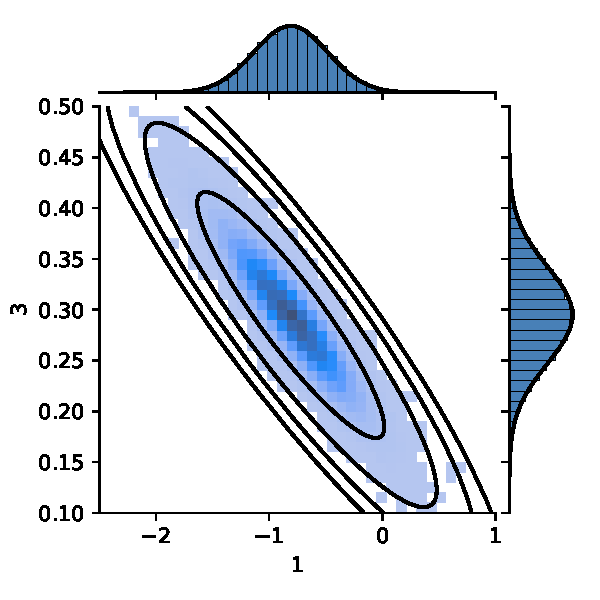
\includegraphics[width=\textwidth]{Figures/simulated_joint_HMC_15.pdf} 
        \caption{HMC conditioned on all datapoints.}
    \end{subfigure}
    \begin{subfigure}[b]{0.4\textwidth}
        \centering
        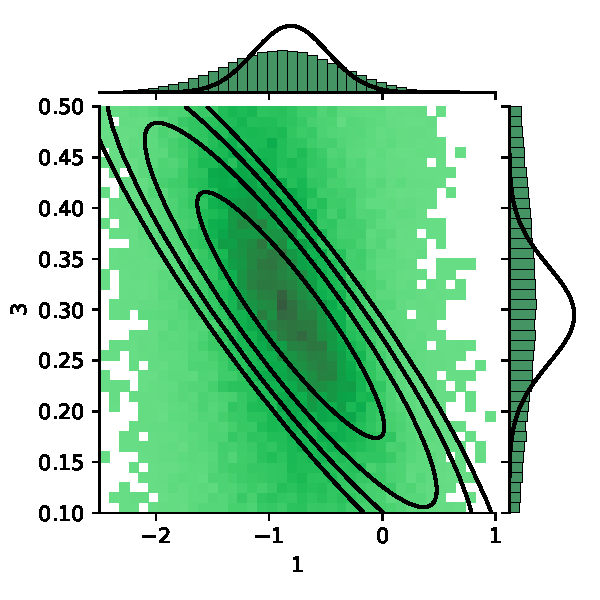
\includegraphics[width=\textwidth]{Figures/simulated_joint_HMC_5.pdf} 
        \caption{HMC with batch size 5}
    \end{subfigure}
    \begin{subfigure}[b]{0.4\textwidth}
        \centering
        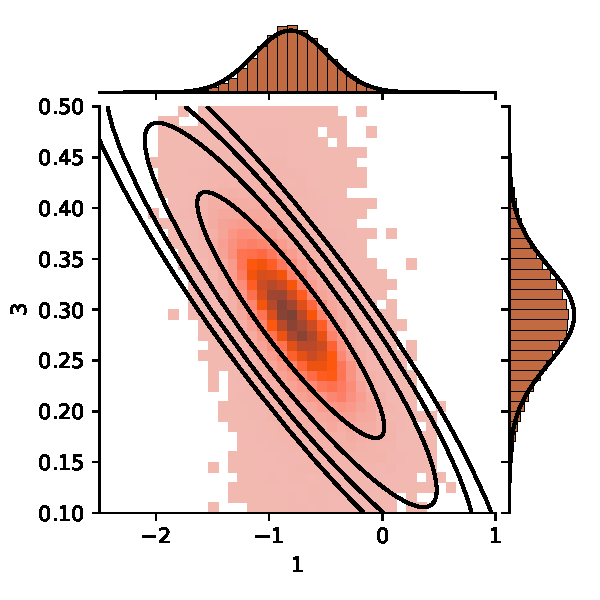
\includegraphics[width=\textwidth]{Figures/simulated_joint_SGHMC_5.pdf} 
        \caption{SGHMC with batch size 5}
    \end{subfigure}
    \caption{Joint distribution of samples for $a_1$ and $a_3$ for the polynomial regression example for HMC and SGHMC for different batch sizes, with the actual posterior density also shown.}
    \label{fig:simulated_joint_comp}
\end{figure}
We find that the also with this approach to the naive SGHMC the batched HMC doesnt, with the sampled posterior having 

with not even the marginal densities being anywhere close to the actual parameter posterior. Notably, the SGHMC seems to provide a more resonable estimate, however still with some overdispersion. In the following section, a possible improvement upon this algorithm is discussed.

